\subsection{Datenmodell}\label{subsec:datenmodell}
Bevor im folgenden Kapitel die Generierung von Dateien erläutert wird, bedarf es der Betrachtung
des Datenmodells, welches aus einer Workflow-Beschreibung entsteht.
Der Inhalt einer Workflow-Beschreibung wird in~\ac{YAML}-Syntax vorgenommen.
Diese wird durch den YAML-Parser von \textit{SnakeYAML}\footnote{\url{https://www.baeldung.com/java-snake-yaml}} in Java-Objekte umgewandelt.
Aus der Liste an Java-Objekten wird das Datenmodell eines~\ac{ES}-Boards erstellt, welches die Generierung von Dateien ermöglicht.
In Abbildung~\ref{fig:classdiagram} ist das Klassendiagramm abgebildet, welches die Struktur eines \ac{ES}-Boards nach dem Parsen der YAML-Eingabe widerspiegelt.

\begin{figure}[h]
    \centering
    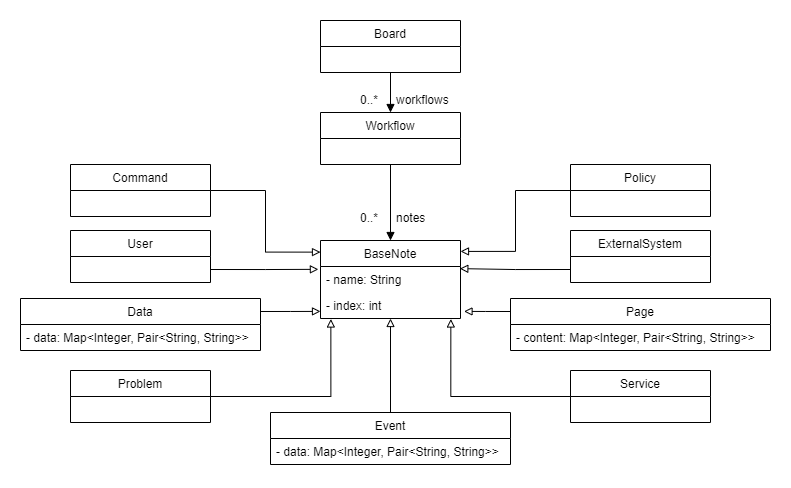
\includegraphics[width=1\textwidth]{images/3.1/classdiagram.drawio}
    \caption{Klassendiagramm fulibWorkflows}
    \label{fig:classdiagram}
\end{figure}

Jeder Note besitzt eine dazugehörige Klasse, welche von BaseNote erbt.
Für jeden Note existiert somit ein Name und ein Index, auf welchen im folgenden Abschnitt eingegangen wird.
Da es im Event Storming ein dazugehöriges \textit{Board} gibt, ist dies ebenfalls eine Klasse, welche alle \textit{workflows} einer Eingabe hält.
Ein Workflow besteht weiterhin aus vielen Notes.
Wie zuvor bereits erläutert, sind Data, Event und Page Sonderfälle unter den Notes, da diese weitere Daten beherbergen.
Daher haben diese Klassen ein Attribut, welches diese Daten organisiert in einer Map hält.
Hierbei wird als key der Index eines Notes verwendet und das value ist ein Pair.
Das Pair beinhaltet den Bezeichner und den dazugehörigen Wert einer zusätzlichen Property eines Notes.
